\documentclass[xcolor=x11names]{beamer}

\usetheme{metropolis}           % Use metropolis them
\usecolortheme{metropolis}

%Defining the theme
% \usetheme{Madrid}
% \useoutertheme[subsection=true,shadow]{miniframes}
%  \useinnertheme{circles}
%  \usepackage{etoolbox}
%  \usepackage{calc}

\definecolor{TaridesDarkBlue}{RGB}{10, 63, 92}
\definecolor{TaridesMidDarkBlue}{RGB}{1, 91, 140} %015B8C
%\definecolor{TaridesMidDarkBlue}{RGB}{2, 113, 168} %0271A8
\definecolor{TaridesMidBlue}{RGB}{3, 150, 216}   % 0396D8
\definecolor{TaridesBrightBlue}{RGB}{55, 180, 236} % 37B4EC
\definecolor{TaridesLightBlue}{RGB}{144, 216, 252} % 90D8FC

% \setbeamercolor{palette primary}{bg=TaridesDarkBlue,fg=white}
% \setbeamercolor{palette secondary}{bg=TaridesLightBlue,fg=white}
% \setbeamercolor{palette tertiary}{bg=TaridesMidBlue,fg=white}
% \setbeamercolor{palette quaternary}{bg=TaridesBrightBlue,fg=white}
%\setbeamercolor{structure}{fg=TaridesDarkBlue} % itemize, enumerate, etc
%\setbeamercolor{section in toc}{fg=TaridesDarkBlue} % TOC sections
%\setbeamercolor*{frametitle}{fg=black,bg=DeepSkyBlue4}
%\setbeamercolor*{lower separation line head}{bg=black}


% Various packages
\usepackage[utf8]{inputenc}
\usepackage[french]{babel}
\usepackage[T1]{fontenc}
\usepackage{lmodern}
\usepackage{enumitem}
\usepackage{amsmath,amssymb,amsfonts}
\usepackage{xcolor}
\usepackage{listings,lstautogobble}
\usepackage{courier}
\lstset{language=caml,autogobble=true,
        commentstyle=\color{TaridesBrightBlue},
        basicstyle=\footnotesize\ttfamily,
        breaklines=true, 
        morekeywords={val},
        morekeywords=[2]{int, string, file_perm, unit, dir_handle, file_descr, open_flag, bytes, bool, option, list},
        keywordstyle=[2]{\color{TaridesMidDarkBlue}}
        }
        
\usepackage{graphicx}
\usepackage{pifont}
\usepackage{hyperref}

\patchcmd{\thebibliography}{\section*{\refname}}{}{}{}

\setbeamertemplate{blocks}[rounded][shadow=true]
\setbeamertemplate{itemize subitem}[bullet]

\newcommand{\added}[1]{\textcolor{gray!60!cyan}{#1}}
\newcommand{\subtt}[1]{\textcolor{gray!30!cyan}{#1}}

\newcommand\wip{\textcolor{red}{Work in progress }}
\newcommand\todo[1]{\textcolor{red}{\textit{\small{#1}}}}

\title[Programmation système en OCaml]{Programmation système en OCaml : introduction et cas d'usage.}
\author[Carine et Lucas]{Carine Morel et Lucas Pluvinage}
\institute{Tarides}

\begin{document}
\maketitle

\begin{frame}{Tarides}

    \begin{itemize}[label=$-$]
        \item on fait des logiciels et du service en OCaml
        \item 70 employés (France, UK, USA, Inde etc..)
        \item tout en open source !  
    \end{itemize}
    
\begin{columns} 
    \column{0.3\linewidth} 
    \centering
    
\includegraphics[width=\textwidth]{slides/images/logo-TARIDES.png}

    \column{0.5\linewidth}
    \centering
    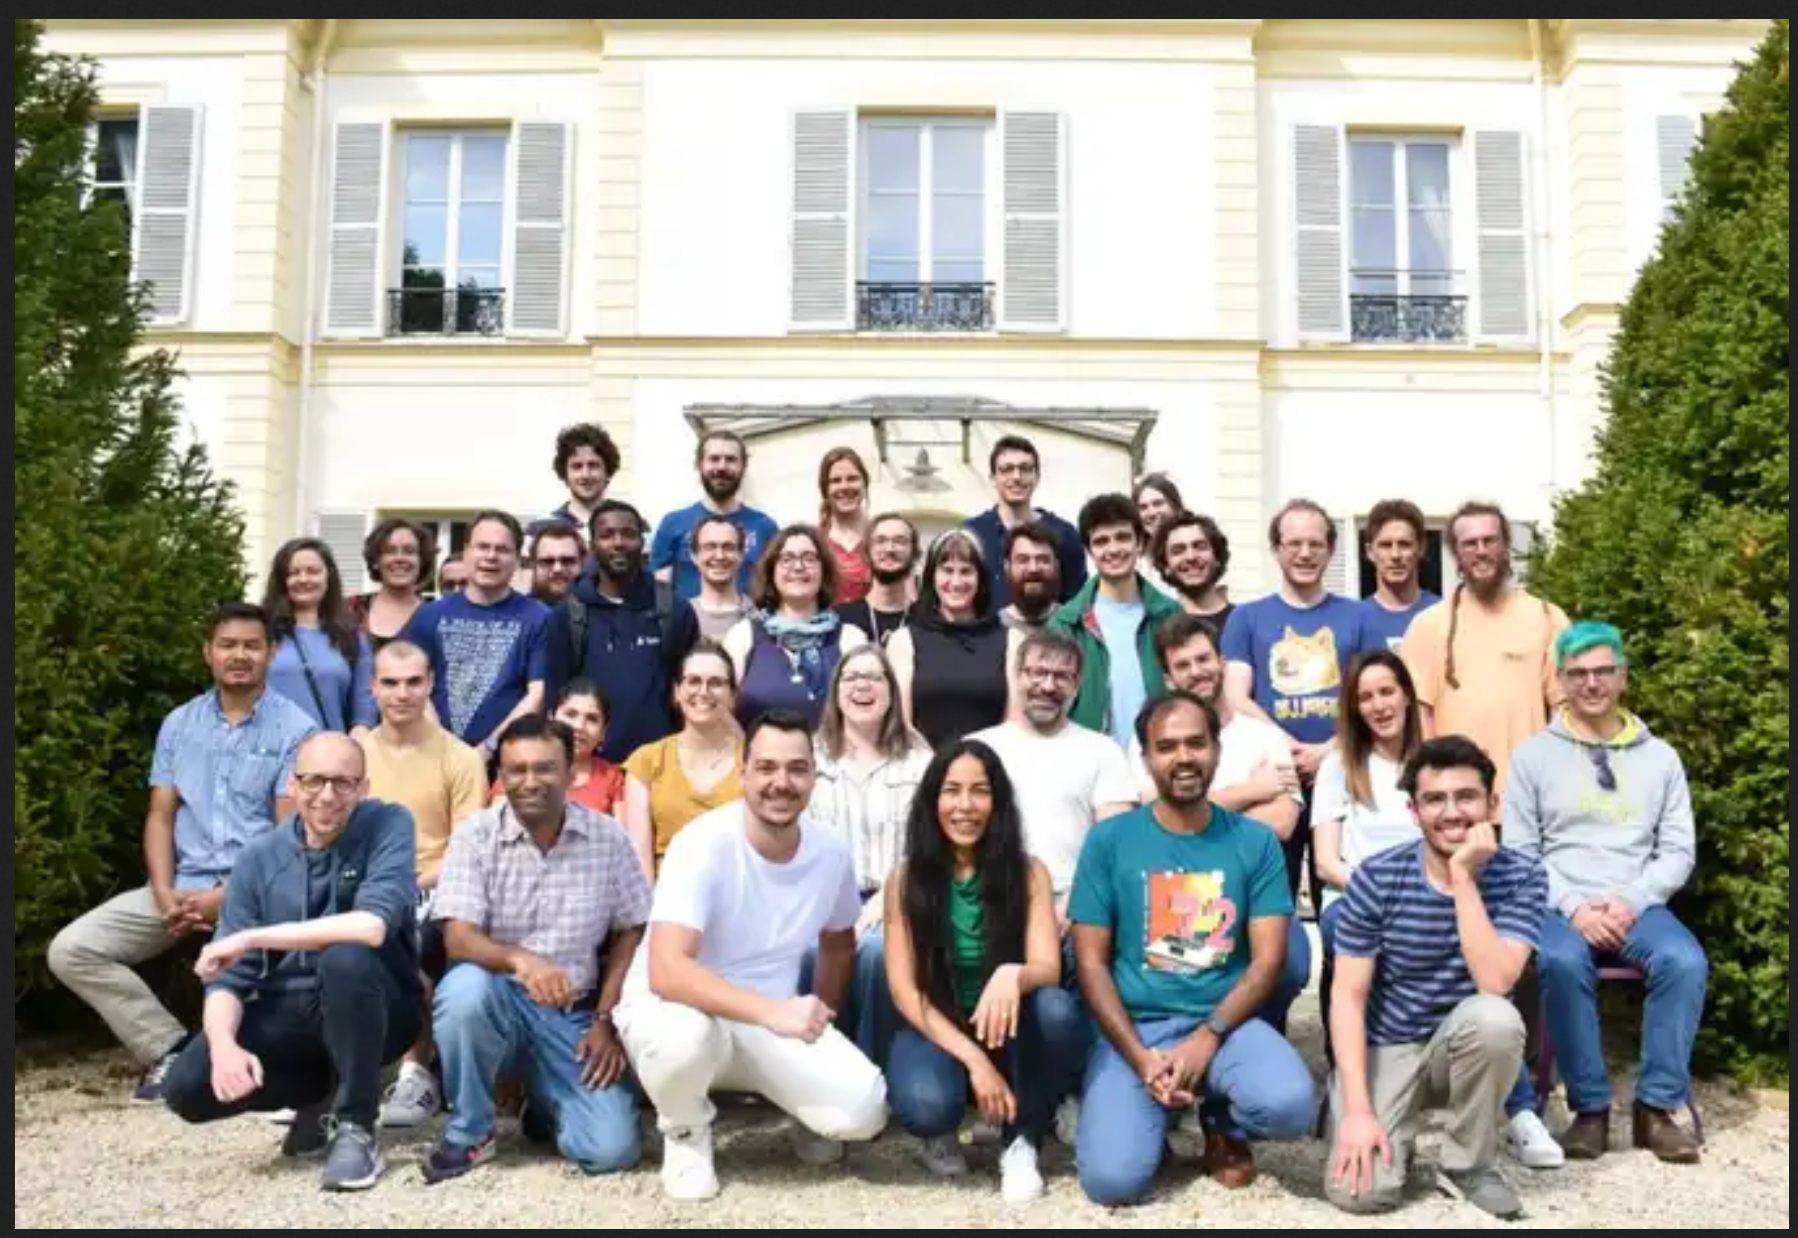
\includegraphics[width=\textwidth]{slides/images/tarides_team.png}
\end{columns}

\end{frame}

\begin{frame}{Plan}
   \subtt{Programmation système en OCaml} 
   
   \ding{217} autour de l'écriture d'un "mini" shell :
    \begin{itemize}[label=\ding{114}]
        \item le module Unix
        \item les processus Unix  
        \item et plus
    \end{itemize}   
    
    \ding{217} les algos d'exclusion mutuelle en OCaml

    \subtt{OCaml dans la vraie vie} 
     \begin{itemize}[label=$-$]
        \item Mirage : \textbf{un} système en OCaml
        \item QCheck : un vérificateur de propriétés automatiques
        \item OCaml 5.0
        \item Écosystème OCaml
    \end{itemize}   
\end{frame}

\section{Programmation système en OCaml}

\subsection{Introduction}

\begin{frame}{Introduction : mini-shell}

    \subtt{Objectif :} programmer un shell en utilisant le module \texttt{Unix} 
    
    \todo{Screenshot d'un shell}
    
    Les fonctionnalités et commandes que l'on va implémenter :
    \begin{itemize}[label=\small\ding{114}]
        \item<1-> Manipulation des fichiers : \texttt{ls}, \texttt{mkdir}, \texttt{ln}, \texttt{cat}
        \item<1-> Modification du répertoire courant : \texttt{cd}
        \item<1-> Processus et environnement % entrée/sortie standard, fork
        \item<1-> Re-directions de flux :  $>$, $<$
        \item<1-> Tube : $|$

        %\item<2-> Pour aller plus loin : 
        %    \begin{itemize}[label=$-$]
        %        \item un peu de \textit{réseau}
        %        \item les sur-couches au module \texttt{Unix} : \textit{Lwt / Bos}
        %    \end{itemize}
    \end{itemize}
\end{frame}

\begin{frame}{Programmation système en OCaml}

    \begin{itemize}[label=\small\ding{114}]
        \item Des modules bas niveau (cf \url{ocaml.org/api})
            \begin{itemize}[label=\small\ding{118}]
                \item \texttt{Sys} : fonctions communes à Unix et aux autres OS sous lesquels tourne OCaml,
                \item \texttt{Unix} : fonctions spécifiques à Unix.
            \end{itemize}
        \item Des sur-couches sur le module \texttt{Unix} :
            \begin{itemize}[label=\small\ding{118}]
                \item certaines fonctions de la \texttt{Sdtlib}, 
                \item \texttt{Lwt.Unix}, 
                \item \texttt{Bos} etc..
            \end{itemize}
        \item Des modules utilitaires comme \texttt{Filename}
    \end{itemize}

\end{frame}

\begin{frame}{Module \texttt{Sys}}
    \begin{itemize}[label=\small\ding{114}]
        \item \wip
    \end{itemize}
\end{frame}

\subsection{Manipulation de fichiers et répertoire}
\begin{frame}[fragile]{Manipulation de fichiers et répertoire : interface du mini-shell}
    \begin{itemize}[leftmargin=-12pt]
    \item<1->Première version de l'AST des commandes :
        \todo{reorganiser dans l'ordre le plus pertinent en fonction de la suite}
        \begin{lstlisting}[breaklines=false]
            type command =
              | Cat of string list           (* cat files *)  
              | Ln of string * string * bool (* ln source dest [-s] *)
              | Mv of string * string        (* mv source dest *)
              | Rm of string * bool          (* rm filename [-r] *)  
              | Mkdir of string * int option (* mkdir dir [-m int] *)
              | Ls of string option          (* ls [filename] *)  
        \end{lstlisting}
        
    \item<2-> Parser, et interpréteur de commandes :
         \begin{lstlisting}
            val parse : string -> command
            val exec_command : command -> unit 
        \end{lstlisting}
    \end{itemize}
\end{frame}  

\begin{frame}[fragile]{Parseur et interpréteur}

    \begin{itemize}[label=\small\ding{114}]
    \item Parseur : plusieurs solutions (\texttt{Args}, \texttt{Angstrom} etc..)
    \item Interpréteur : 
      \begin{lstlisting}
            let exec_command cmd = 
                match cmd with
                | Cat filename              -> failwith "todo"
                | Ln (source, dest, symb)   -> failwith "todo"
                | Mv (source, dest)         -> failwith "todo"
                | Mkdir (dirname, perm_opt) -> failwith "todo"
                | Rm (filename, recursive)  -> failwith "todo"
                | Ls name_opt               -> failwith "todo"
        \end{lstlisting}
    \end{itemize}
\end{frame} 


\input{slides/systeme_3_réseau}

\begin{frame}[fragile]{Interactions haut niveau avec le système}
 
\subtt{Le module \texttt{Stdlib} contient des primitives haut niveau pour la manipulation de fichiers}

\begin{lstlisting}
type in_channel
type out_channel

val open_in : string -> in_channel
val input_line : in_channel -> string
val close_in : in_channel -> unit

val open_out : string -> out_channel
val output_string : out_channel -> string -> unit
val close_out : in_channel -> unit

\end{lstlisting}
    
\end{frame}

\begin{frame}{Programmation asynchrone}
Plusieurs stratégies:
\begin{itemize}
    \item Utiliser des fils d'exécution (threads)
    \item \texttt{Lwt}: bibliothèque pour fils d'exécutions légers
\end{itemize}
\end{frame}

\begin{frame}[fragile]{Exemple: \texttt{cp} asynchrone avec \texttt{Lwt\_unix}}

\begin{lstlisting}
let rec perform_copy_lwt src dst =
  let* n = Lwt_unix.read src buffer 0 buf_size in
  if n = buf_size then
    let* _ = Lwt_unix.write dst buffer 0 n in
    perform_copy_lwt src dst
  else
    let* _ = Lwt_unix.write dst buffer 0 n in
    Lwt.return (`Ok ())

let cp_lwt src dest =
  Lwt_main.run @@
  let* fd_src = Lwt_unix.openfile src [O_RDONLY] 0 in 
  let* fd_dst = Lwt_unix.openfile dest [O_RDWR; O_CREAT; O_TRUNC] 0o640 in
  perform_copy_lwt fd_src fd_dst
\end{lstlisting}
    
\end{frame}


\begin{frame}{OCaml IRL}

\begin{enumerate}[label=\small\ding{114}]
    \item MirageOS: un système d'exploitation modulaire écrit en OCaml
    \item OCaml 5: programmation parallèle (et effets)
    \item QCheck: vérification de propriétés automatique
    \item Écosystème et environnements de programmation
\end{enumerate}
    
\end{frame}


\begin{frame}{MirageOS}
    
\begin{figure}
    \centering
    \begin{minipage}{0.45\textwidth}
        \centering
        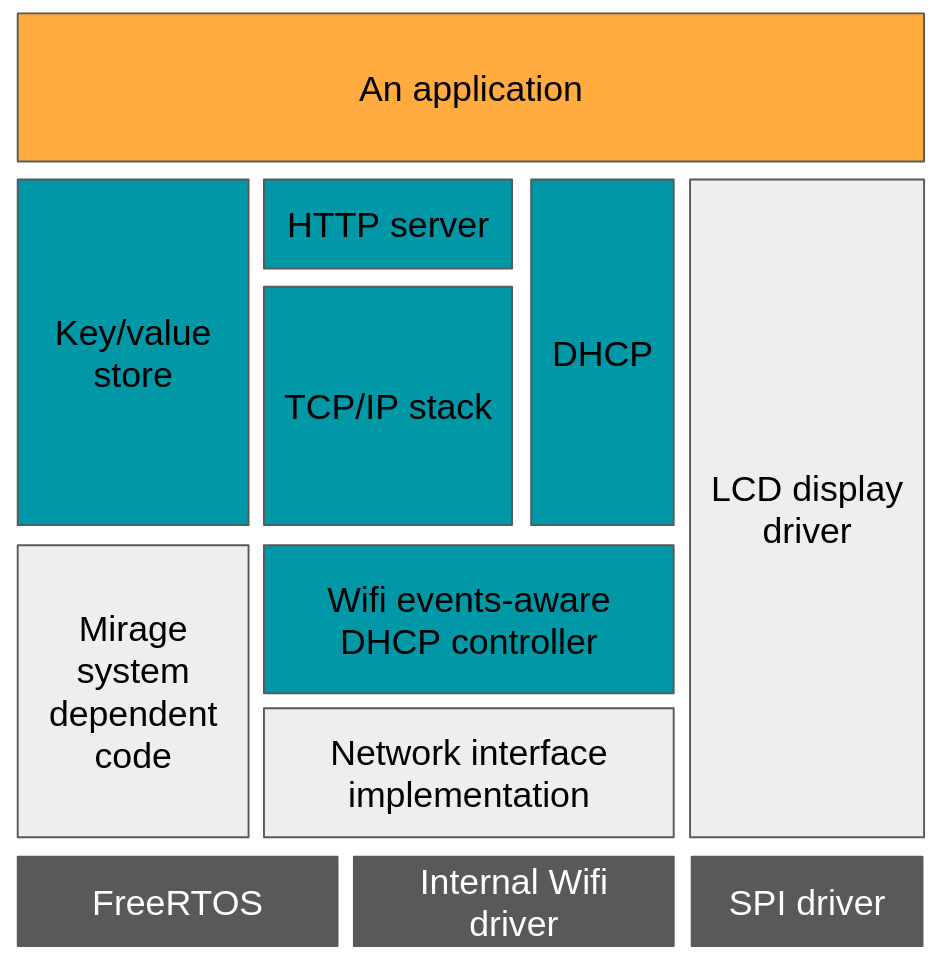
\includegraphics[width=0.9\textwidth]{slides/images/mirage.png}
        \caption{Une application modulaire}
    \end{minipage}\hfill
    \begin{minipage}{0.45\textwidth}
        \centering
        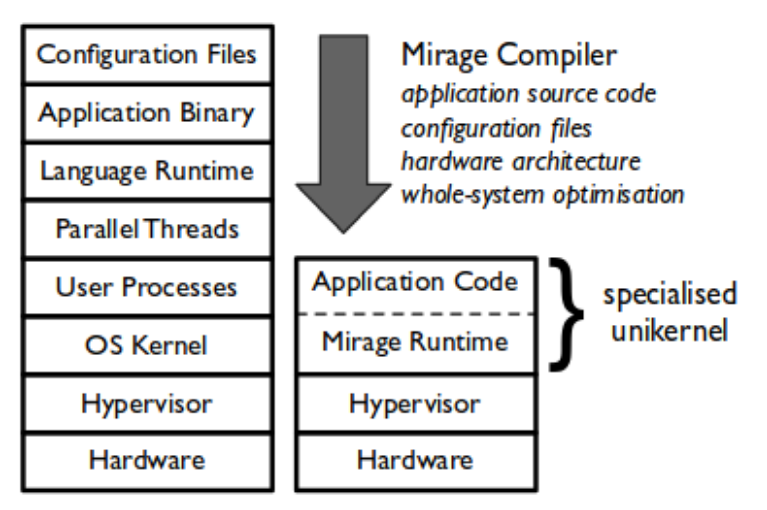
\includegraphics[width=0.9\textwidth]{slides/images/mirage2.png}
        \caption{MirageOS compile à la fois l'application et le système dans un seul exécutable}
    \end{minipage}
\end{figure}

\end{frame}

\begin{frame}[fragile]{Abstraction: signatures de modules}

\begin{lstlisting}
module type Read_only_store = sig 
    type t
    type key = string
    
    val get : t -> key -> string Lwt.t
end
\end{lstlisting}

\begin{lstlisting}
module type HTTP = sig
    type t
    module Request : sig 
        type t
        
        val path : t -> string
    end
    type reponse = string
    
    val listen : t -> (HTTP.Request.t -> response Lwt.t) -> unit Lwt.t
end
\end{lstlisting}


\end{frame}

\begin{frame}[fragile]{Implémentation}
    
\begin{lstlisting}

(* les dependances de notre application sont abstraites 
   via le foncteur Make *)
module Make (FS : Read_only_store) (Server : HTTP) = 
struct
    let start fs http =
        HTTP.listen http (fun request ->
            let path = HTTP.Request.path request in
            FS.get fs path)
end

(* pour les tests *)
module Application = Make (In_memory_store) (Mock_http_server)

(* en production *)
module Application = Make (EXT4) (Cohttp.Server)
\end{lstlisting}

\end{frame}

\begin{frame}{Modules disponibles}
\begin{enumerate}[label=$-$]
    \item Socket réseau: TCP/IP de l'OS ou en OCaml
    \item Stockage: en mémoire, Irmin, FAT
    \item Protocoles: Git, HTTP, SSH, DNS, DHCP
    \item Cryptographie / compression
\end{enumerate}
\end{frame}

%\begin{frame}[fragile]{Boucle d'événements}
%
%\begin{lstlisting}
%val run : unit Lwt.t -> unit
%\end{lstlisting}
%
%\begin{lstlisting}
% let run t =
%   let rec aux () =
%     Time.restart_threads Time.time;
%     match Lwt.poll t with
%     | Some () -> ()
%     | None ->
%         let timeout = Time.select_next () in
%         let ready_set = solo5_yield timeout in
%         (if ready_set <> 0L then
%          (* Some I/O is possible, wake up threads and continue. *)
%          wakeup_threads ready_set);
%         aux ()
%   in
%   aux ()
% \end{lstlisting}
% \end{frame}


\begin{frame}{OCaml 5}


\begin{figure}
    \centering
    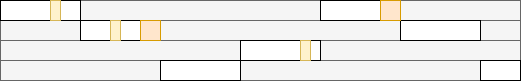
\includegraphics[width=0.9\textwidth]{slides/images/concurrence.png}
    \caption{Concurrence}
\end{figure}

\begin{figure}
    \centering
    \includegraphics[width=0.9\textwidth]{slides/images/parallélisme.png}
    \caption{Parallélisme}
\end{figure}
% Blanc = code OCaml
% Jaune = minor GC
% Orange = major GC
\end{frame}

\begin{frame}{Peterson}
    
\end{frame}

\begin{frame}{Lamport}
    
\end{frame}


\begin{frame}[fragile]{QCheck}
    
Vérification de propriétés

\begin{figure}
    \centering
    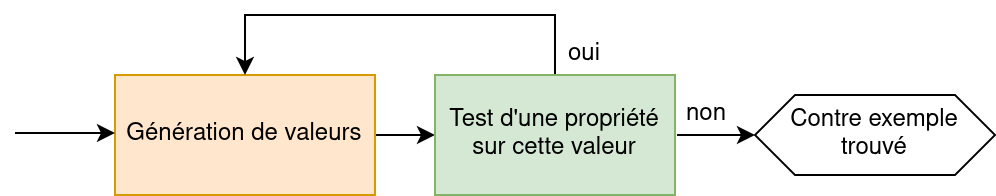
\includegraphics[width=0.9\textwidth]{slides/images/qcheck.drawio.png}
\end{figure}

\subtt{QCheck cherche un contre exemple minimal}

\begin{lstlisting}
type 'a generator
val small_int : int generator
val small_list : 'a generator -> 'a list generator
val Test.make : 'a generator -> ('a -> bool) -> Test.t
\end{lstlisting}

Plus d'informations: \url{https://github.com/c-cube/qcheck}
\end{frame}

\begin{frame}[fragile]{Exemple de test}

\begin{lstlisting}

let generateur = QCheck.(small_list small_int)
\end{lstlisting}

\subtt{Inverser une liste}
\begin{lstlisting}
let predicat entree sortie =
    let entree = Array.of_list entree in
    let sortie = Array.of_list sortie in
    let n = Array.length entree in
    assert (n = Array.length sortie);
    for i = 0 to n - 1 do
      assert (entree.(i) = sortie.(n-1-i))
    done;
    true
\end{lstlisting}

\subtt{Trier une liste}
\begin{lstlisting}
let predicat entree sortie =
    List.sort Int.compare entree = sortie
\end{lstlisting}

\end{frame}

\begin{frame}[fragile]{Réduction}
    
\begin{lstlisting}
  let inverser lst = 
    if List.length lst >= 5 then lst
    else List.rev lst
\end{lstlisting}
\subtt{Réduction du contre exemple}
\begin{lstlisting}
0   => [3176607639030078719; -702777917135807191; 1243225506173352439; -168141035741141589; 4478591693389419378; -2908482084465810011; -4471604993596125836; 2097048314685490782; -777119667999583759]
1   => [1243225506173352439; -168141035741141589; 4478591693389419378; -2908482084465810011; -4471604993596125836; 2097048314685490782; -777119667999583759]
200 => [0; 0; 0; 4095797489620100; -777119667999583759]
255 => [0; 0; 0; 0; -194279916999895940]
299 => [0; 0; 0; 0; -11044]
313 => [0; 0; 0; 0; -1]
\end{lstlisting}

\end{frame}

\begin{frame}{Simulation d'un état}

\begin{figure}
\centering
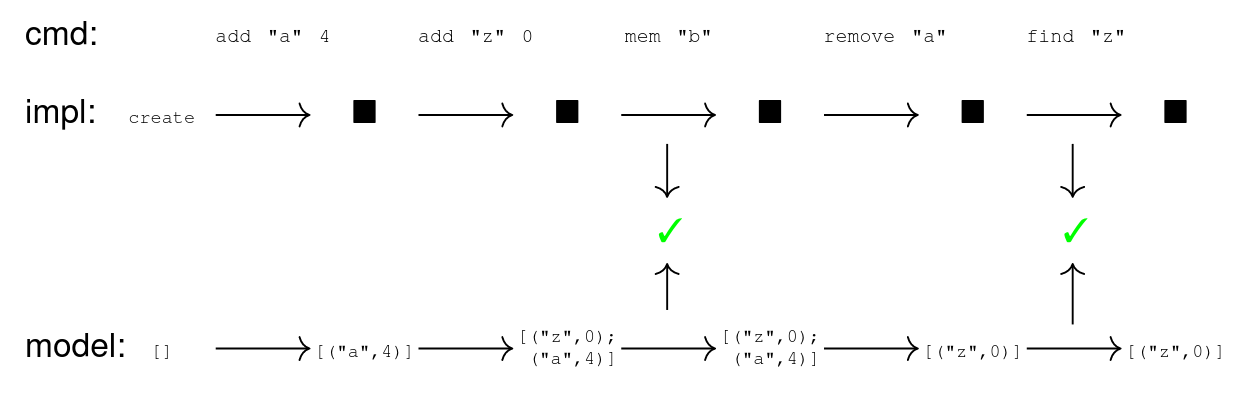
\includegraphics[width=\textwidth]{slides/images/qcheck_state.png}
\end{figure}
\begin{figure}
\centering
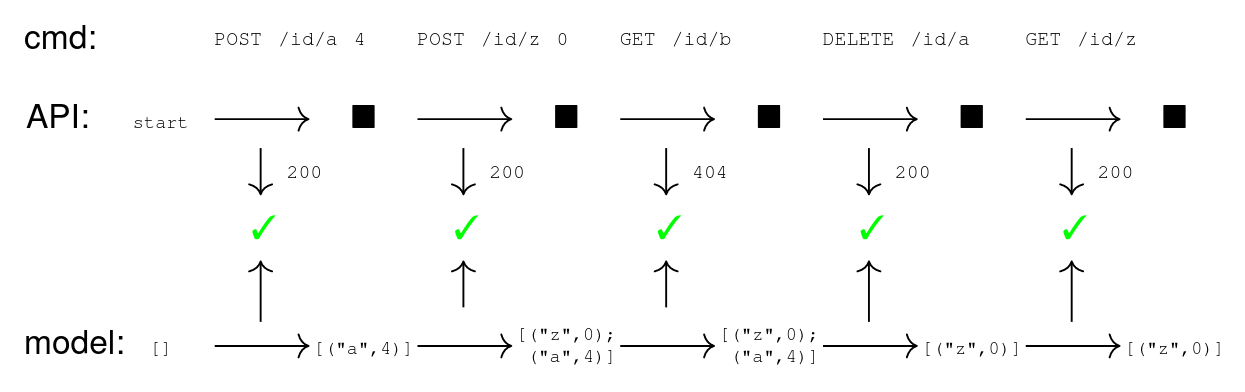
\includegraphics[width=\textwidth]{slides/images/qcheck_state_2.png}
\end{figure}

\end{frame}
\input{slides/irl_4_ecosystème}

\end{document}
